\section{Autora rezultātu dalība konferencēs}
\begin{itemize}
\item Zinātniski praktisks seminārs "Ceļā uz gandrīz nulles enerģijas ēkām (gNEĒ) Latvijā". \emph{LU eksperimentālā poligona monitoringa jaunumi: energoefektivitāte un solārā enerģija}. Rīga, Latvija, 2019.g. 11. aprīlis (prezentācija).
% autors: Viktorija Leimane; prezentēja: Andris Jakovičs
\item 7th European conference on renewable energy systems. \emph{The role of solar panel arrangement on their efficency in typical for Latvia weather conditions}. 2019. g. 10.--12. jūnijs, Madride (prezentācija).
\end{itemize}

\section{Autora ieguldījums darbā}
% the \\ insures the section title is centered below the phrase: Appendix B

Saules paneļu uzstādīšanu veica SIA EG Inženieri Valda Gailīša vadībā.
Par datu ievākšanu no saules paneļu sistēmas datu uzkrājējiem jāpateicas Victron Energy B.V. izstrādātājai Victron Remote Management Portal (VRM) sistēmai.

Mans ieguldījums ir koda arhitektūras plānošana, rakstīšana un uzturēšana līdz šim brīdim. Esmu vienīgais koda bāzes izstrādātājs. Darbā kopā veikti 318 iesūtījumi (\textit{commits}) trīs zaros (105, 123 un 90 iesūtījumi attiecīgi), kas rezultējās 3140 koda rindās. 

Darba gaitā veicu datu lejupielādi, datu informācijas aptveršanu, kā arī datu programmatisku atlasīšanu, apstrādi, apkopošanu, transformēšanu vizualizācijas vajadzību pielāgošanai un datu vizualizāciju. 

\begin{figure}[h]
	\centering
	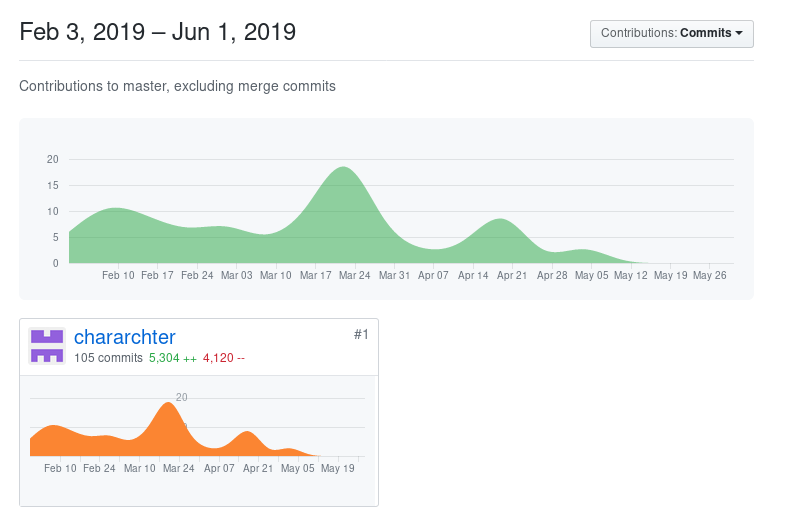
\includegraphics[width=0.6\linewidth]{figures/misc/contributions.png}
	\caption{Darba autores ieguldījums master zarā.}
	\label{fig:retribution}
\end{figure}

% 105 commits master
% 123 commits february
% 90 commits march